\section{Diagramas de flujo}
Con el objetivo de representar de manera detallada la secuencia operativa interna de este sistema, se emplea un diagrama de flujo, el cual describe los procesos, decisiones y ciclos que se ejecutan desde la activación del sistema hasta la llegada al destino.

\begin{figure}[H]
    \centering
    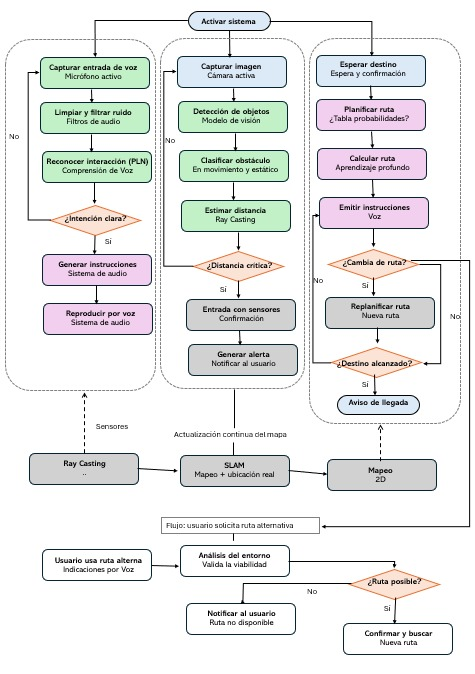
\includegraphics[width=13cm]{DiagFlujo/FlujoGeneral.jpeg}
    \caption{Diagrama de flujo global del sistema}
    \label{fig:flujo_gen}
\end{figure}
\textbf{Módulo 1 - Voz}
El sistema comienza capturando la entrada del usuario mediante el bloque “Capturar entrada de voz”, donde se utiliza el micrófono para recibir comandos. Posteriormente, la señal pasa por el proceso de “Limpiar y filtrar ruido”, en el cual se aplican técnicas de procesamiento de audio para mejorar la calidad de la señal.
\\
Una vez depurada, la información es interpretada en “Reconocer interacción (PLN)”, donde se emplean modelos de procesamiento de lenguaje natural para comprender la intención del usuario.
\\
Se presenta una decisión clave: “¿Intención clara?”.
\\
Si la respuesta es afirmativa, el sistema procede a “Generar instrucciones” y posteriormente a “Reproducir por voz”, proporcionando retroalimentación auditiva al usuario.
En caso contrario, el sistema puede requerir nueva entrada o repetir el proceso de interpretación.
\\
Este módulo es fundamental, ya que permite una interacción natural y accesible entre el usuario y el sistema.

\textbf{Módulo 2 - Visión}
\\
De manera paralela, el sistema activa la cámara en el bloque “Capturar imagen”, obteniendo información visual del entorno. Esta información es procesada en “Detección de objetos”, donde un modelo de visión identifica elementos relevantes.
\\
Posteriormente, en “Clasificar obstáculo”, el sistema determina si los objetos detectados representan un riesgo, diferenciando entre obstáculos móviles y estáticos.
\\
El siguiente paso es “Estimar distancia”, donde se calcula la proximidad de los objetos mediante técnicas como Ray Casting.
\\
Esto conduce a la decisión “¿Distancia crítica?”:
\\
Si se detecta un riesgo cercano, el sistema ejecuta “Entrada con sensores” para validar la información y posteriormente “Generar alerta”, notificando al usuario.
Si no existe riesgo, el sistema continúa monitoreando el entorno sin interrumpir la navegación.
\\
Este módulo garantiza la seguridad del usuario mediante análisis en tiempo real del entorno.

\textbf{Módulo 3 - Ruta}
En este módulo, el sistema puede encontrarse inicialmente en el estado “Esperar destino”, hasta recibir la confirmación del usuario. Una vez definido, se ejecuta “Planificar ruta”, donde se evalúan posibles trayectorias.
\\
Posteriormente, en “Calcular ruta”, se emplean algoritmos de aprendizaje profundo para determinar la mejor opción disponible. El resultado se comunica mediante “Emitir instrucciones”, guiando al usuario durante su desplazamiento.
\\
Durante la navegación, el sistema evalúa continuamente la condición “¿Cambia de ruta?”:
\\
Si no hay cambios, el sistema sigue emitiendo instrucciones.
Si ocurre un evento (por ejemplo, un obstáculo), se activa “Replanificar ruta”, generando una nueva trayectoria.
\\
Finalmente, se evalúa “¿Destino alcanzado?”:
\\
Si la respuesta es afirmativa, el sistema ejecuta “Aviso de llegada”, concluyendo el proceso.
En caso contrario, el ciclo de navegación continúa.

\textbf{Sensores y mapeo}
Se presenta:
SLAM (Mapeo y ubicación en tiempo real)
Mapeo 2D
Ray Casting
\\
Estos elementos permiten la actualización continua del entorno, proporcionando información clave a los módulos de visión y planificación. Gracias a este sistema, el modelo puede tomar decisiones informadas en tiempo real.
\\
Se contempla un flujo adicional cuando el usuario decide cambiar la ruta. Este proceso inicia en “Usuario usa ruta alterna”, seguido de un “Análisis del entorno” para validar la viabilidad.
\\
Se evalúa la decisión “¿Ruta posible?”:
\\
Si la ruta es viable, el sistema procede a “Confirmar y buscar nueva ruta”.
En caso contrario, se ejecuta “Notificar al usuario ruta no disponible”, informando la imposibilidad del cambio.
\subsection{Flujo de percepción}
Para los modulos que ayudan al sistema a percibir el mundo como el de Visión y el de los sensores, el flujo es:
El proceso interno del sistema para la detección, análisis y validación de obstáculos, integrando información proveniente de visión por computadora y sensores físicos. Su objetivo principal es garantizar que las decisiones de navegación se basen en información confiable, reduciendo falsos positivos y aumentando la seguridad del usuario.
\begin{figure}[H]
    \centering
    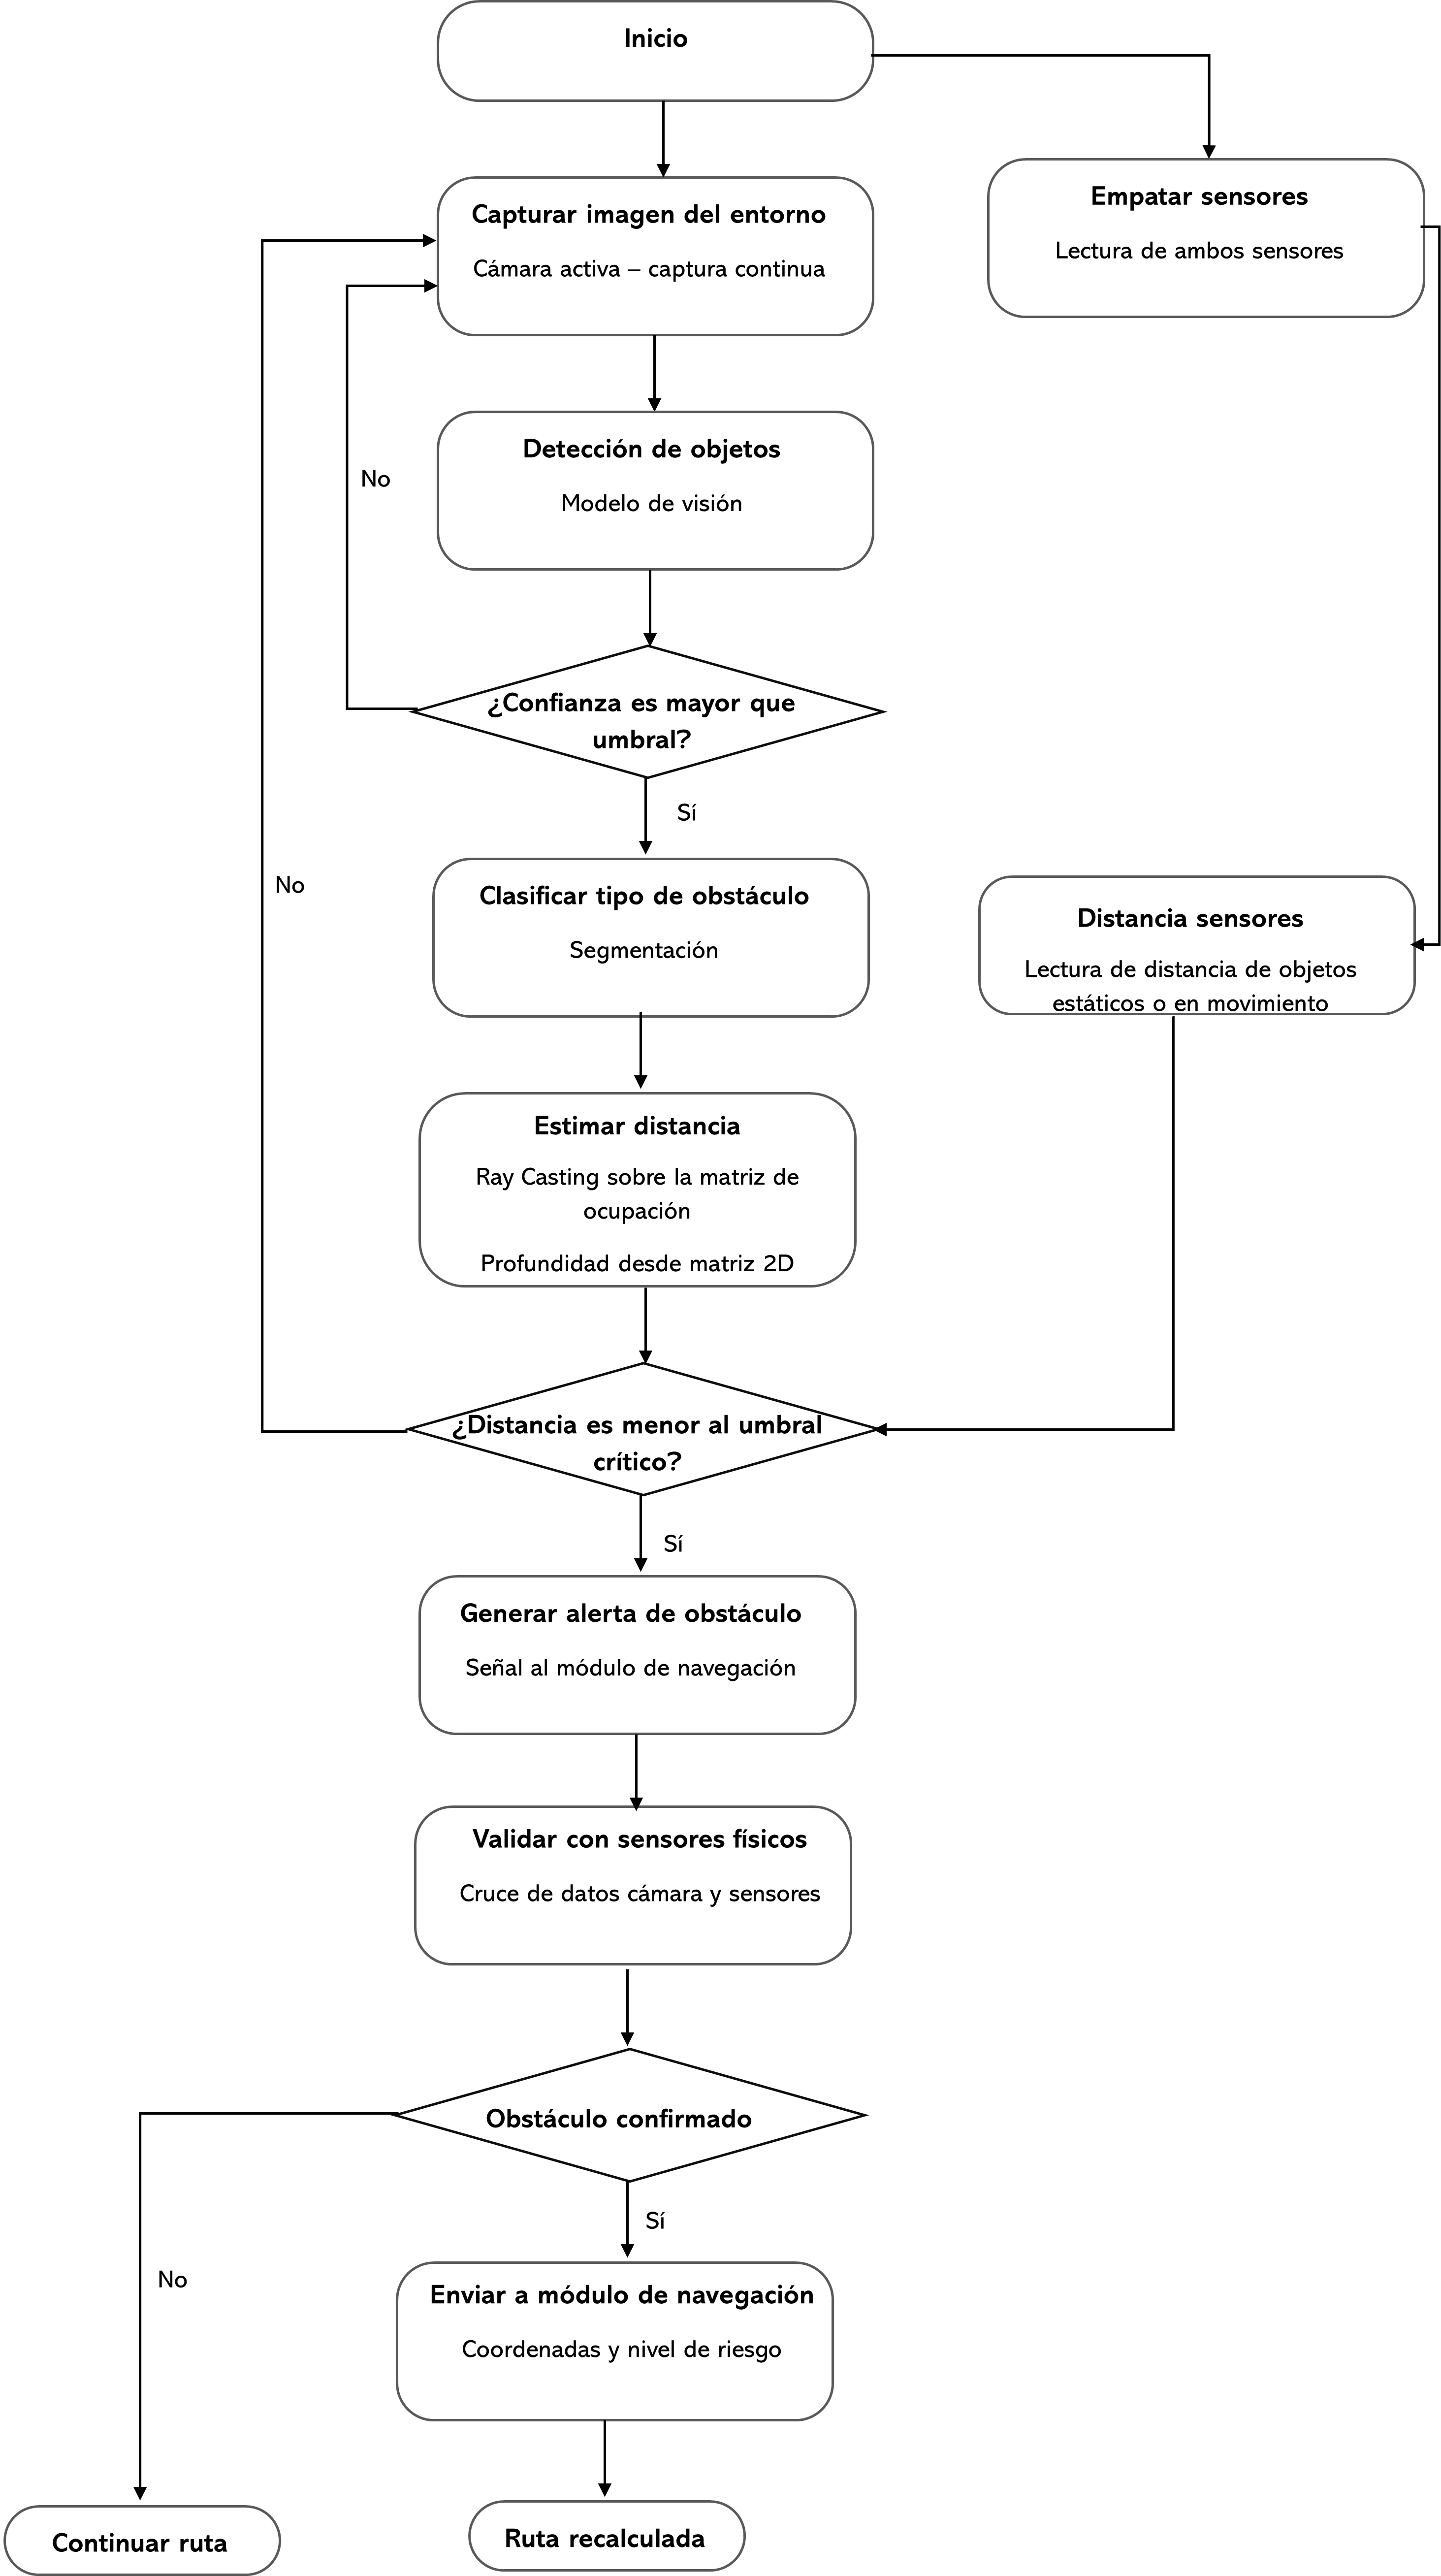
\includegraphics[width=11cm]{DiagFlujo/FlujoVision.png}
    \caption{Diagrama de flujo del Modulo de Vision y Modulo sensorial}
    \label{fig:flujo_vision}
\end{figure}
El flujo inicia a partir de dos procesos fundamentales:
Captura de imagen mediante una cámara activa y la entrada de los sensores, donde se realiza la lectura simultánea de los sensores físicos para sincronizar la información.

Una vez capturada la imagen, el sistema ejecuta el proceso de “Detección de objetos”, utilizando un modelo de visión por computadora para identificar elementos presentes en el entorno.

Posteriormente, se evalúa la condición “¿Confianza es mayor que umbral?”, la cual determina si la detección es suficientemente confiable:
Si la confianza no supera el umbral, el sistema descarta la detección y regresa al proceso de captura.
Si la confianza es adecuada, el flujo continúa con el análisis del objeto detectado.

Cuando la detección es válida, el sistema procede a “Clasificar tipo de obstáculo”, diferenciando entre objetos estáticos y dinámicos mediante técnicas de segmentación.
“Estimar distancia”, utiliza Ray Casting  sobre los objetos.

Los sensores físicos aportan información mediante el bloque “Distancia sensores”, proporcionando una medición adicional independiente de la visión.
Con la información obtenida, se evalúa la condición “¿Distancia es menor al umbral crítico?”:
Si no se encuentra dentro de un rango de riesgo, el sistema continúa monitoreando sin generar intervención.
Si la distancia es crítica, se activa el proceso de respuesta.

En este caso, el sistema ejecuta “Generar alerta de obstáculo”, enviando una señal al módulo de navegación para advertir la presencia de un posible riesgo.

“Validar con sensores físicos”, donde se cruzan los datos obtenidos por la cámara y los sensores.
A continuación, se evalúa la decisión “Obstáculo confirmado”:
Si no se confirma, el sistema descarta la alerta y continúa con la navegación normal.

Una vez validado el obstáculo se ejecuta “Enviar a módulo de navegación”, proporcionando las coordenadas del obstáculo y nivel de riesgo.

Con esta información, el sistema de navegación puede tomar decisiones informadas, como ajustar la trayectoria y recalcular la ruta.

Esto se refleja en el resultado “Ruta recalculada”. En caso de que no se confirme el obstáculo, el flujo concluye en “Continuar ruta”, manteniendo la trayectoria actual.

\subsection{Flujo de Navegación}
En este diagrama se explica el flujo de la navegación que se llevará a cabo.

\begin{figure}[H]
    \centering
    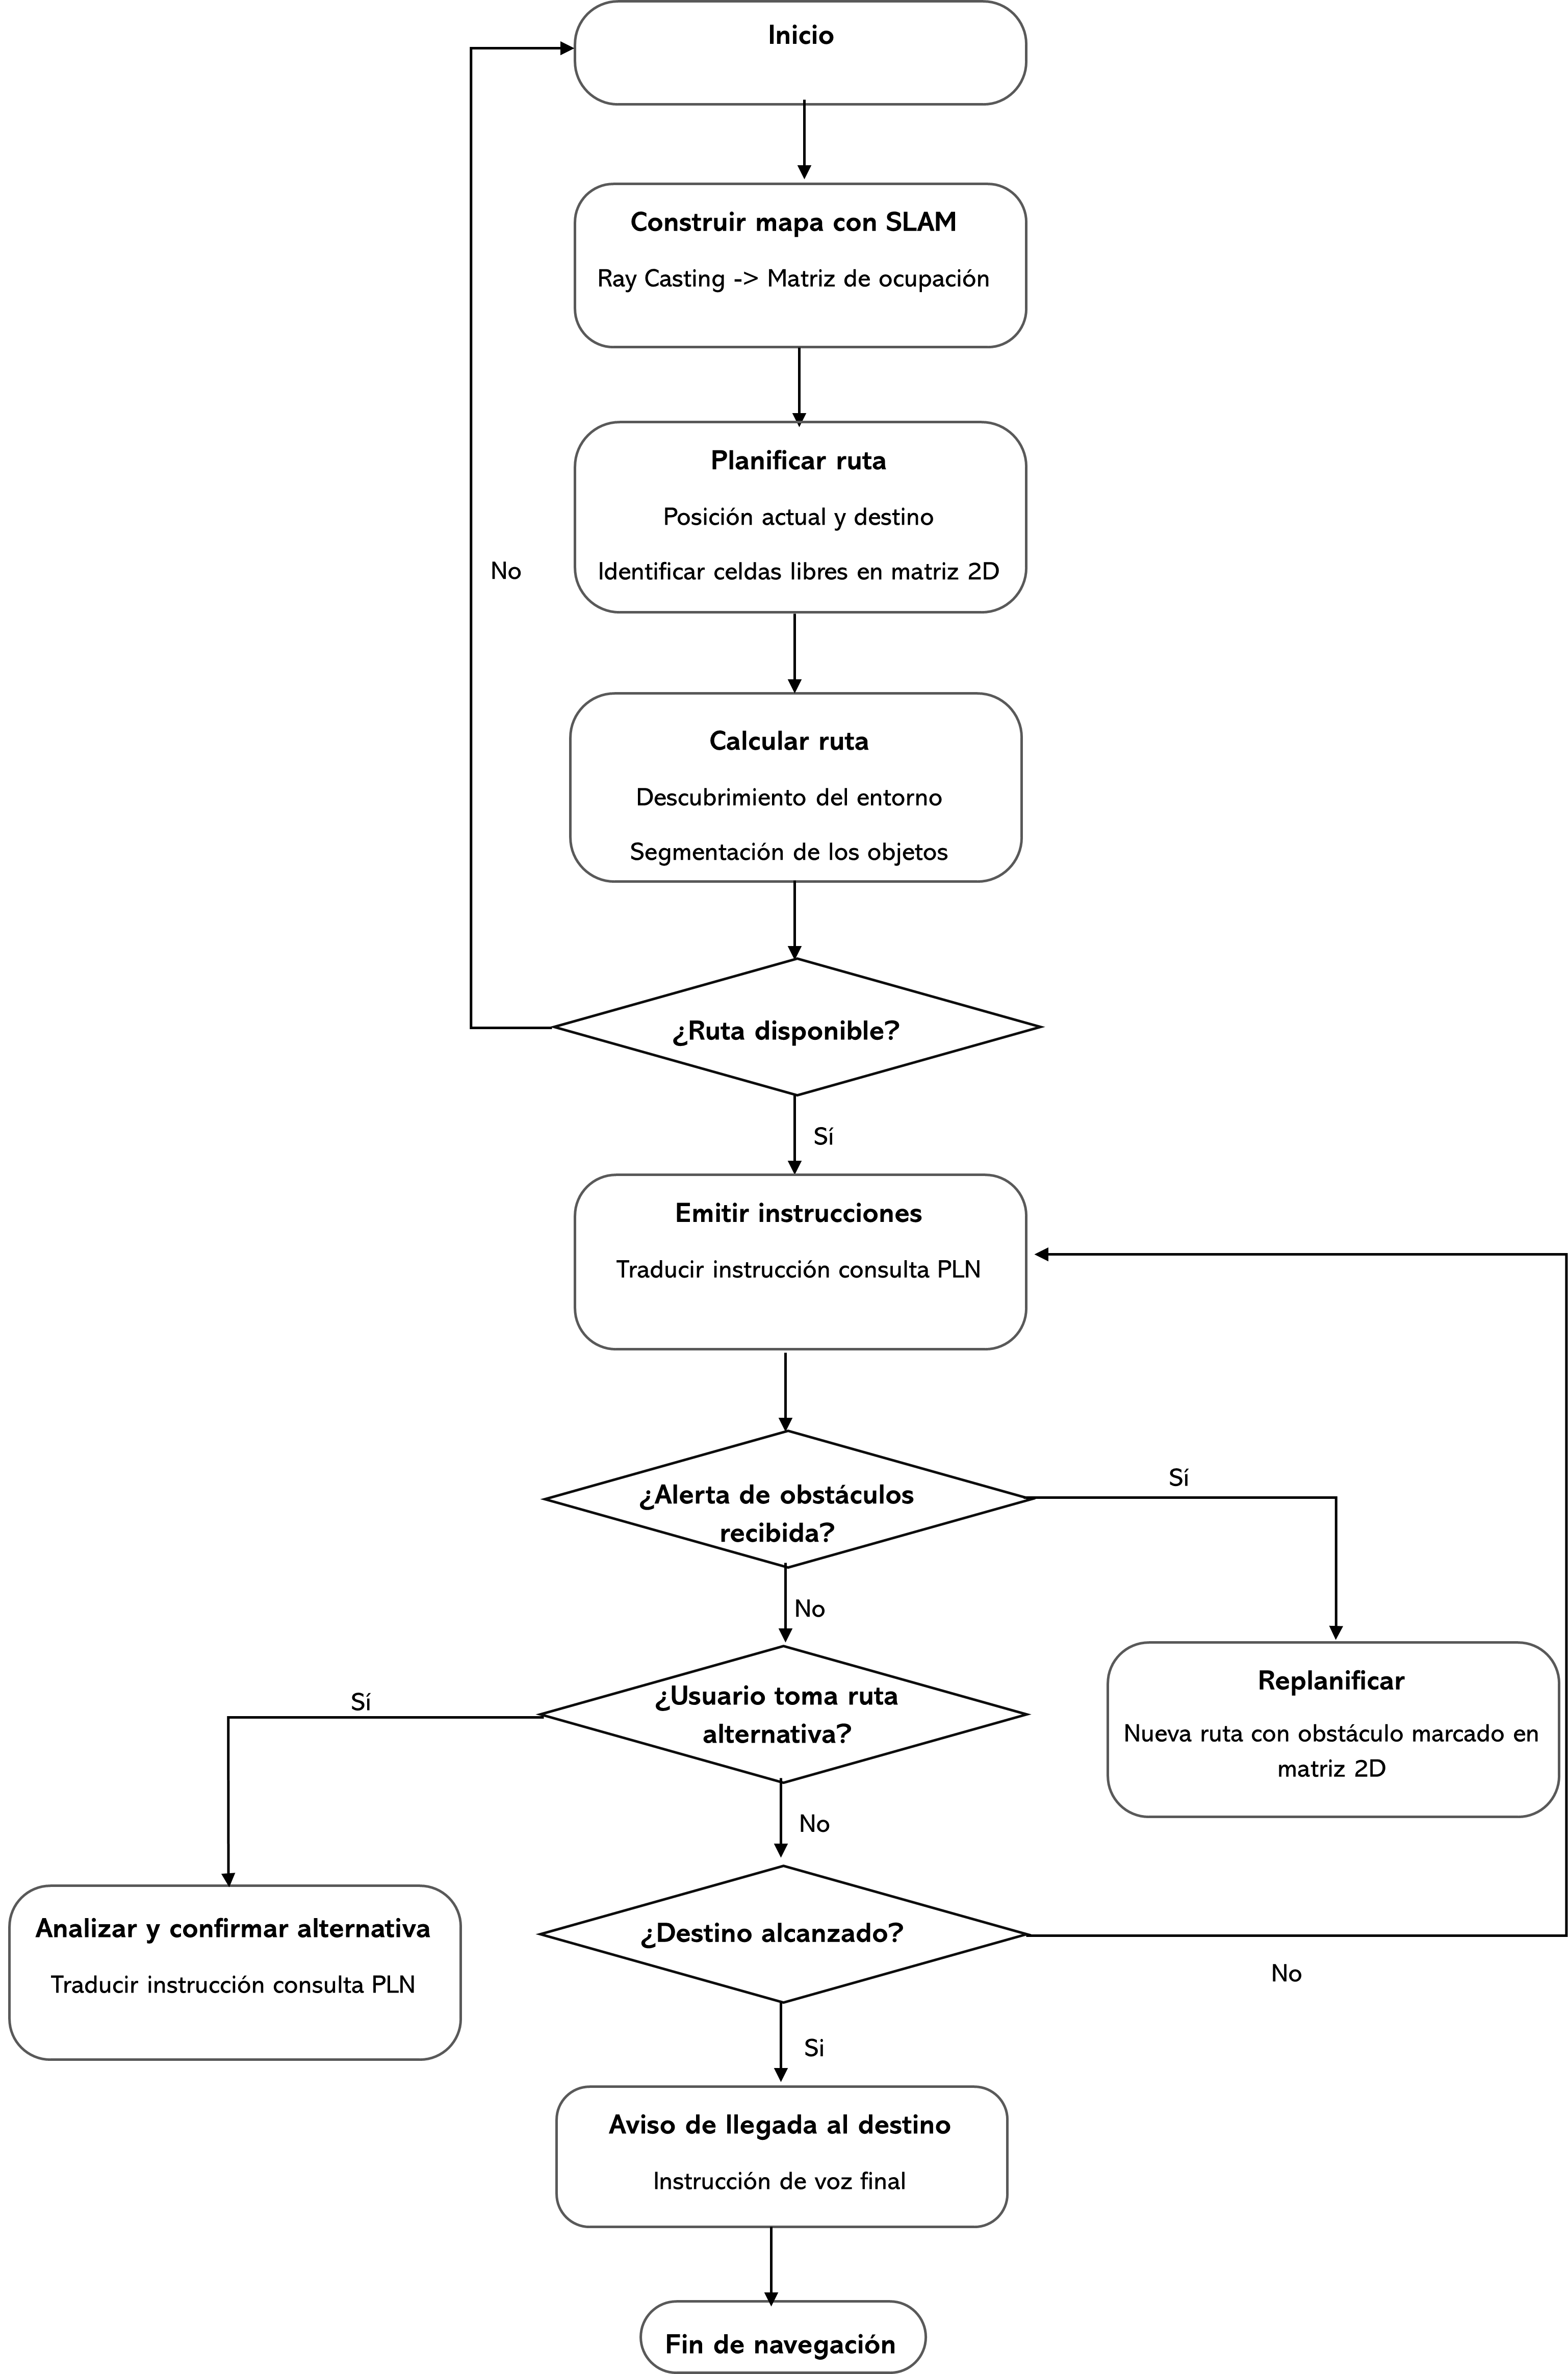
\includegraphics[width=11cm]{DiagFlujo/FlujoNavegacion.png}
    \caption{Diagrama de flujo del Modulo de Visión y Modulo sensorial}
    \label{fig:flujo_nav}
\end{figure}
El flujo inicia en el bloque Inicio y avanza hacia la construcción del entorno espacial mediante SLAM (Simultaneous Localization and Mapping), donde el sistema aplica Ray Casting para generar una matriz de ocupación 2D.

Con el mapa listo, el sistema ejecuta la planificación de ruta, identificando la posición actual, el destino y las celdas libres en la cuadrícula. 

A partir de esto, calcula la ruta mediante descubrimiento del entorno y segmentación de objetos. Si no existe una ruta disponible, el flujo regresa a planificar nuevamente. Cuando sí hay una ruta, se evalúa la condición ¿Ruta disponible? y el sistema procede a emitir instrucciones traducidas mediante procesamiento de lenguaje natural (PLN).

Desde ese punto se abre un ciclo de navegación activa:
Si llega una alerta de obstáculo, el sistema pasa a Replanificar, marcando el obstáculo en la matriz 2D y generando una nueva ruta, para luego volver a emitir instrucciones.

Si no hay alerta pero el usuario toma una ruta alternativa, el sistema la analiza y confirma mediante PLN.

Si no hay alerta y el usuario sigue la ruta, se evalúa si el destino fue alcanzado: si no, el ciclo regresa a emitir instrucciones; si sí, se emite un aviso de llegada por voz y el flujo concluye en Fin de navegación.

\subsection{Flujo de la Interacción}
Aquí se muestra como se comporta el flujo de los módulos de Reconocimiento de Voz, PLN y salida al usuario, permitiendo la interacción natural entre el usuario y el sistema de navegación asistida.

\begin{figure}[H]
    \centering
    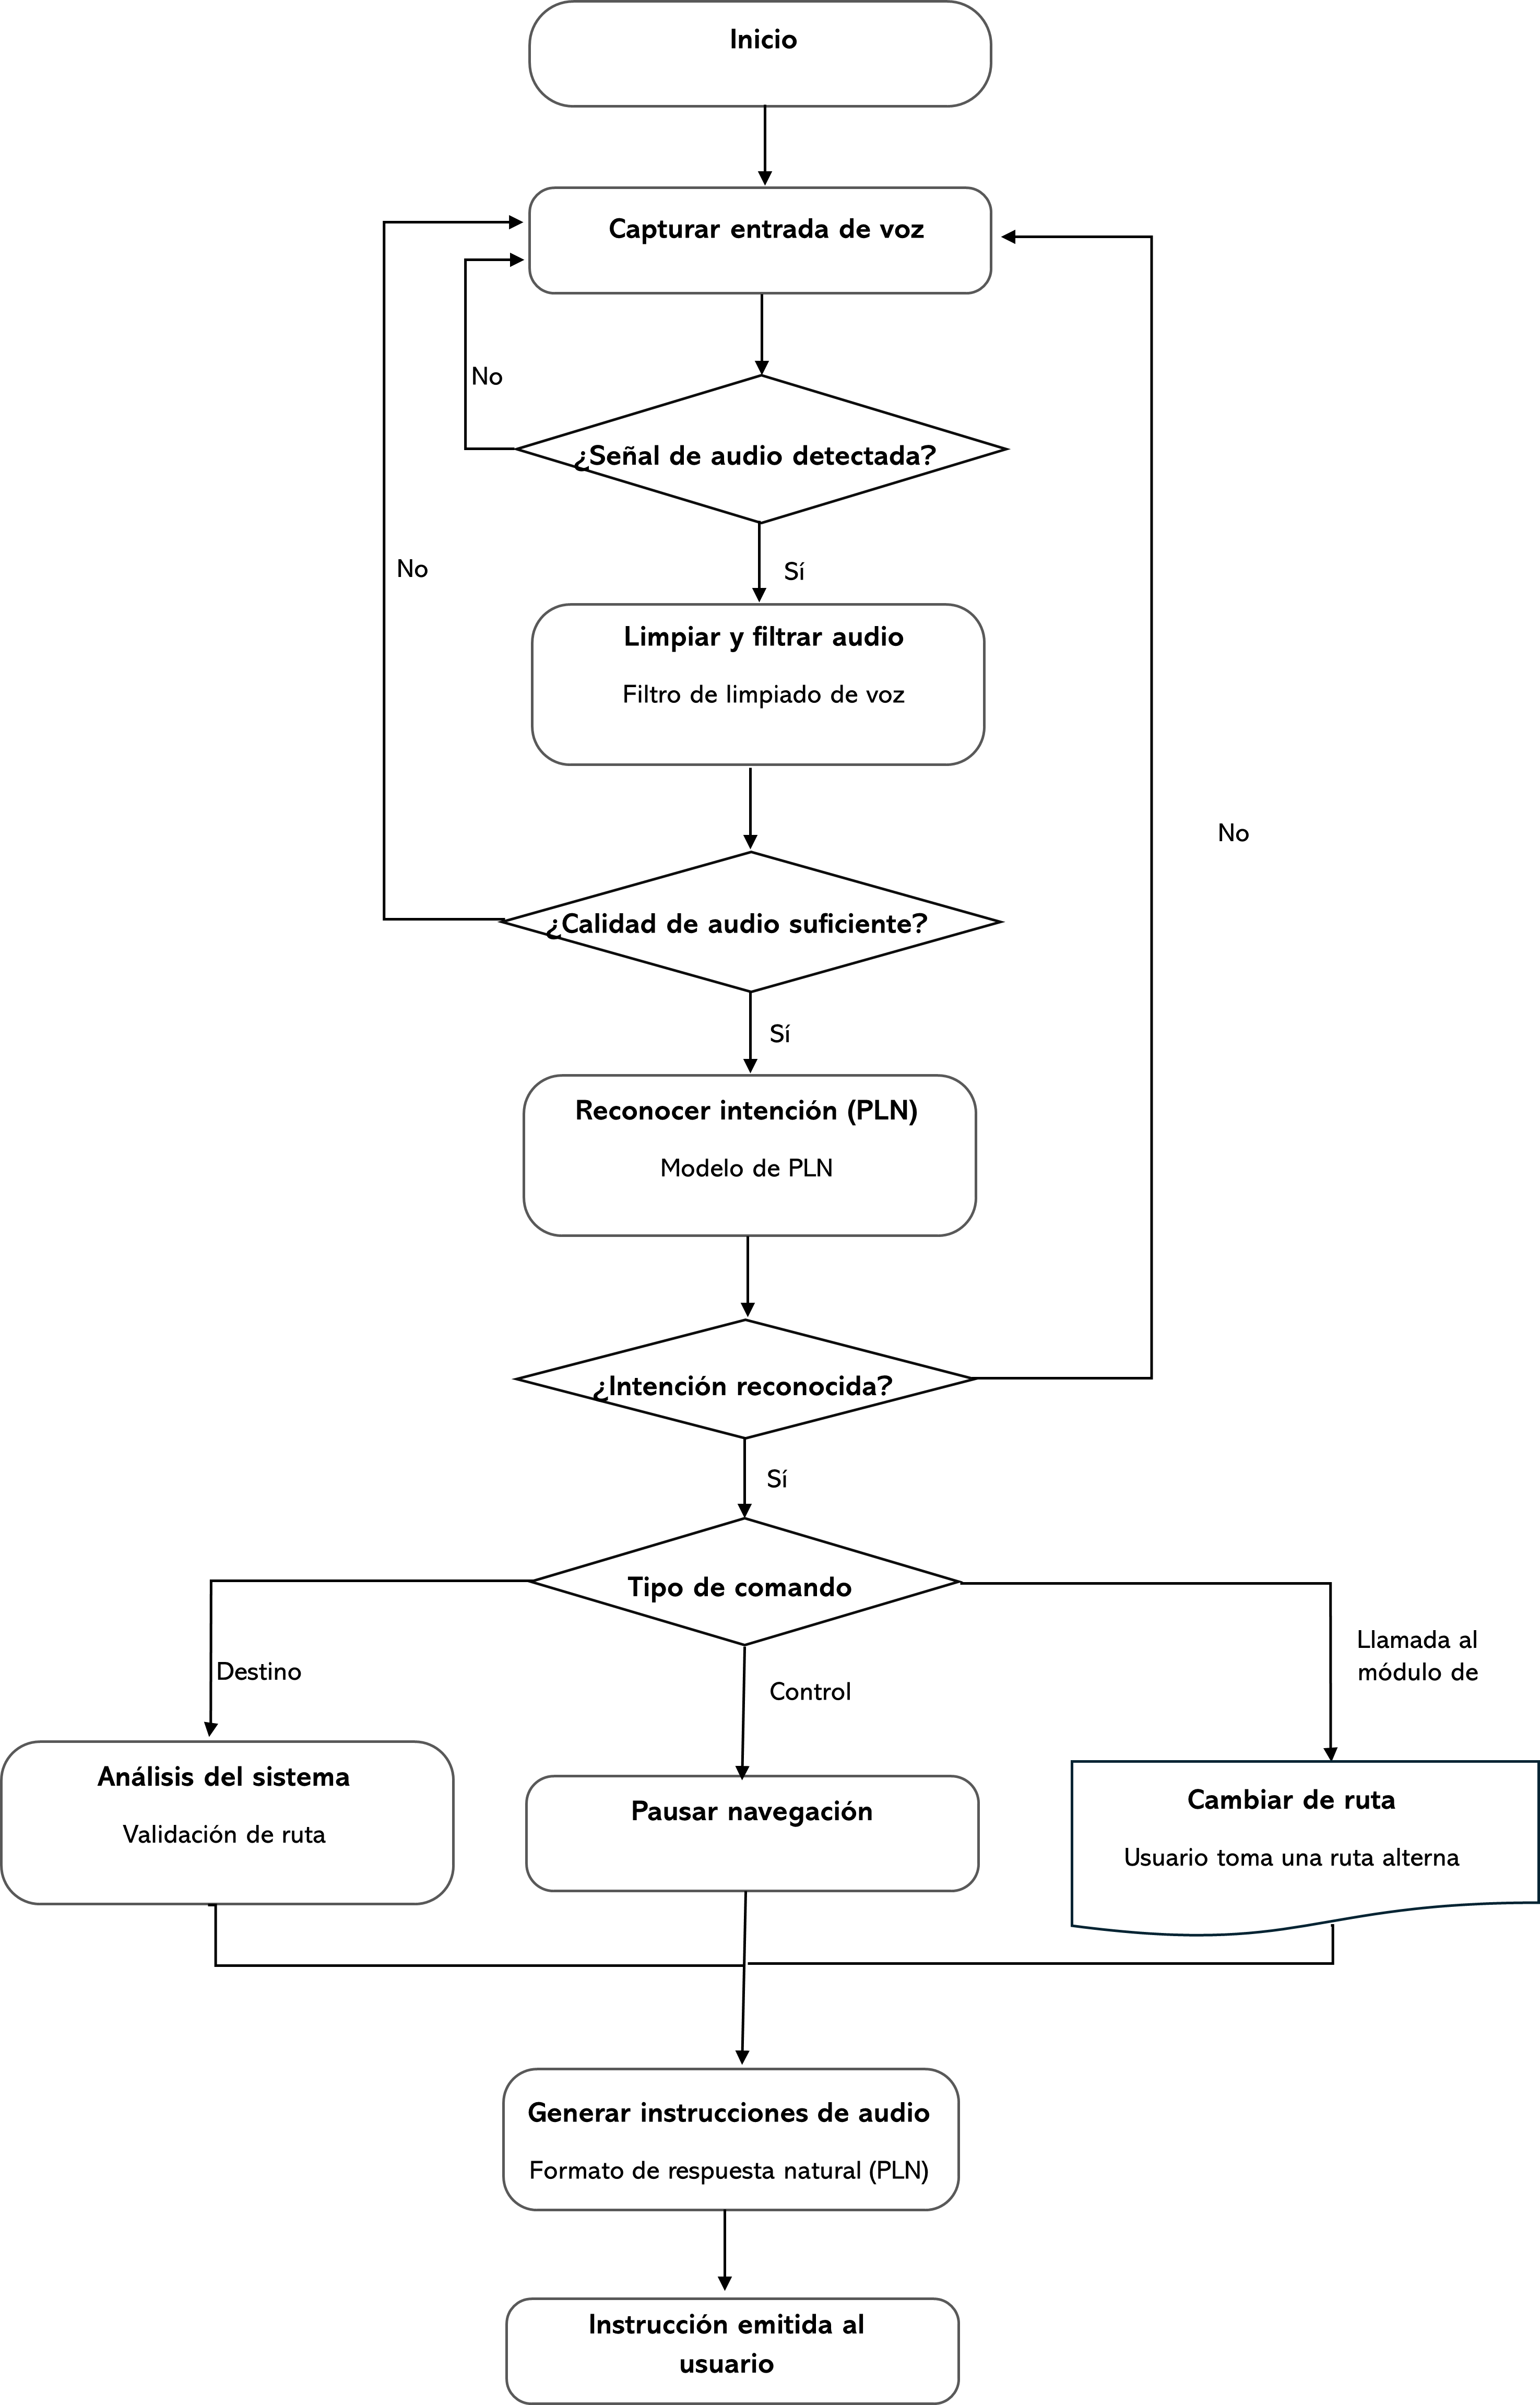
\includegraphics[width=11cm]{DiagFlujo/FlujoVozPLN.png}
    \caption{Diagrama de flujo del Modulo de Lenguaje Natural y Reconocimiento de voz}
    \label{fig:flujo_pln}
\end{figure}
El proceso inicia en el bloque “Inicio”, seguido de “Capturar entrada de voz”, donde el sistema activa el micrófono para adquirir señales de audio de manera continua.
Se evalúa la condición “¿Señal de audio detectada?”:
Si no se detecta señal, el sistema permanece en estado de espera y continúa monitoreando la entrada de audio.
Si se detecta señal, el flujo avanza al procesamiento de la misma.

Una vez detectada la señal, el sistema ejecuta el bloque “Limpiar y filtrar audio”, donde se aplican técnicas de reducción de ruido y mejora de calidad.
Se evalúa “¿Calidad de audio suficiente?”:
Si la calidad no es adecuada, el sistema descarta la señal y regresa a la captura, evitando interpretaciones erróneas.
Si la calidad es suficiente, el flujo continúa hacia el análisis semántico.
Este paso es fundamental para garantizar la confiabilidad del reconocimiento.

El sistema procesa la señal mediante el bloque “Reconocer intención (PLN)”, utilizando un modelo de procesamiento de lenguaje natural para interpretar el contenido del mensaje y se evalúa la condición “¿Intención reconocida?”:
Si no se reconoce la intención, el sistema vuelve al estado de captura, solicitando implícitamente una nueva entrada.
Si la intención es reconocida, el flujo continúa hacia la clasificación del comando.

Una vez comprendida la intención, el sistema clasifica la solicitud en el bloque “Tipo de comando”, distinguiendo tres puntos principales:
\begin{enumerate}
    \item Comandos de destino: Se dirigen al bloque “Análisis del sistema”, donde se realiza la validación de la ruta hacia el destino solicitado. Este proceso implica verificar la viabilidad del trayecto y preparar la navegación.
    \item Comandos de control: Incluyen acciones como “Pausar navegación”, permitiendo al usuario modificar el estado del sistema en tiempo real.
    \item Cambio de ruta: Corresponde al bloque “Cambiar de ruta”, donde el usuario solicita una alternativa. Este caso implica la comunicación con el módulo de navegación para recalcular el trayecto.
\end{enumerate}
Independientemente del tipo de comando, el sistema procede al bloque “Generar instrucciones de audio”, donde se construye una respuesta en lenguaje natural mediante técnicas de PLN.

Finalmente, se ejecuta “Instrucción emitida al usuario”, proporcionando retroalimentación auditiva clara y comprensible.